\normaltrue \difficilefalse \tdifficilefalse
\correctiontrue
%\UPSTIidClasse{11} % 11 sup, 12 spé
%\newcommand{\UPSTIidClasse}{11}

\exer{Exercice $\star$ \label{PERF:06:C2:03:prec:64}}
%% CCP MP 2007
\setcounter{question}{0}\marginnote{\xpComp{PERF}{06}}%\UPSTIcompetence[2]{C2-03}
\index{Compétence C2-03}
\index{Schéma-blocs}
\index{Précision}

\ifcorrection
\marginnote{\textbf{Corrigé à vérfier.}}
\else
\marginnote{\textbf{Pas de corrigé pour cet exercice.}}
\fi


\ifprof
\else
On donne le système suivant dont la la FTBF est donnée par 
$G(p)=\dfrac{\Theta_S(p)}{\Theta_C(p)}=\dfrac{3,24}{p^2+3,24 p+3,24}$. Le retard du système est de \SI{0,2}{s}.

L'asservissement est donné par le schéma-blocs suivant.

\begin{marginfigure}
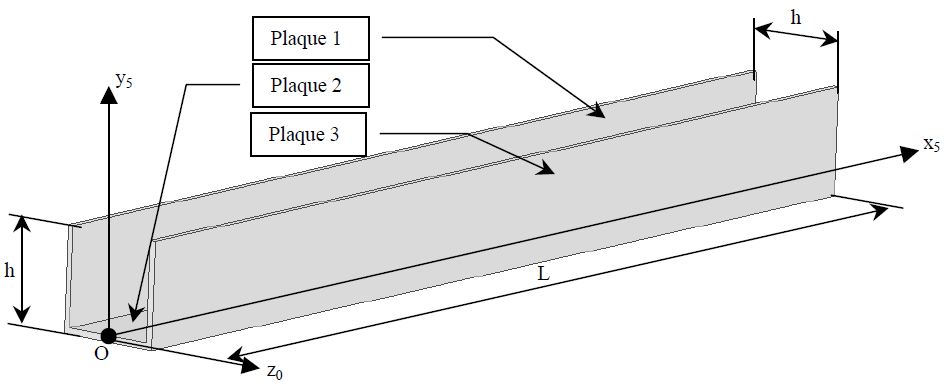
\includegraphics[width=\linewidth]{64_01}
\end{marginfigure}

\fi

 
\question{En considérant le retard nul, déterminer l'écart statique.}
\ifprof

La boucle fermée est de gain unitaire. On a donc $\varepsilon_S = 0$.
\else 
\fi

\question{En considérant le retard nul, déterminer l'expression de la boucle ouverte $H_{\text{BO}}(p)$.}
\ifprof

On a $G(p)=\dfrac{F(p)}{1+F(p)}$ avec $F(p)$ la FTBO. On donc $G(p)+G(p)F(p)=F(p)$ et
 $F(p)=\dfrac{G(p)}{1-G(p)} $
 $ = \dfrac{\dfrac{3,24}{p^2+3,24 p+3,24}}{1-\dfrac{3,24}{p^2+3,24 p+3,24}} $
  $ = \dfrac{3,24}{p\left(p+3,24\right)} $. 

\else 
\fi
 
\question{Déterminer l'expression de $G_r(p)$, transmittance en boucle fermée du système avec retard de \SI{0,2}{s}.}
\ifprof

On a $G_r(p)=\dfrac{\indice{H}{BO}(p)e^{-0,2 p}}{1+\indice{H}{BO}(p)e^{-0,2 p}}$ 
$=\dfrac{\dfrac{3,24}{p\left(p+3,24\right)}e^{-0,2 p}}{1+\dfrac{3,24}{p\left(p+3,24\right)}e^{-0,2 p}}$
$=\dfrac{3,24e^{-0,2 p}}{p\left(p+3,24\right)+3,24e^{-0,2 p}}$.
\else 
\fi


 
\question{Donner la valeur de l'écart statique du système avec retard.}
\ifprof

On a $\lim\limits_{t\to +\infty} \varepsilon(t) $
$= \lim\limits_{p\to 0} p\varepsilon(p) $
$= \lim\limits_{p\to 0} p\left( \Theta_C(p) - \Theta_S(p) \right) $
$= \lim\limits_{p\to 0} p\left( \dfrac{1}{p}-\dfrac{1}{p} G_r(p) \right) $
$= \lim\limits_{p\to 0}  1-\dfrac{3,24e^{-0,2 p}}{p\left(p+3,24\right)+3,24e^{-0,2 p}} $
$= \lim\limits_{p\to 0}  \dfrac{p\left(p+3,24\right)}{p\left(p+3,24\right)+3,24e^{-0,2 p}} $ $=0$.

\else 
\fi
 
Le système est soumis à une rampe de \SI{0,1}{rad.s^{-1}}.
\question{Donner la valeur de l’erreur de traînage correspondant à cette entrée.}
\ifprof

On a $\lim\limits_{t\to +\infty} \varepsilon(t) $
$= \lim\limits_{p\to 0} p\varepsilon(p) $
$= \lim\limits_{p\to 0} p\left( \Theta_C(p) - \Theta_S(p) \right) $
$= \lim\limits_{p\to 0} p\left( \dfrac{0,1}{p^2}-\dfrac{0,1}{p^2} G_r(p) \right) $
$= \lim\limits_{p\to 0}  \dfrac{0,1}{p}\left(1-\dfrac{3,24e^{-0,2 p}}{p\left(p+3,24\right)+3,24e^{-0,2 p}} \right) $
$= \lim\limits_{p\to 0}  \dfrac{0,1}{p}\dfrac{p\left(p+3,24\right)+3,24e^{-0,2 p}-3,24e^{-0,2 p}}{p\left(p+3,24\right)+3,24e^{-0,2 p}}  $
$= \lim\limits_{p\to 0}  \dfrac{0,1}{p}\dfrac{p\left(p+3,24\right)}{p\left(p+3,24\right)+3,24e^{-0,2 p}}  $
$= \lim\limits_{p\to 0}  0,1\dfrac{\left(p+3,24\right)}{p\left(p+3,24\right)+3,24e^{-0,2 p}}  $
$=  0,1 $
\else 
\fi

 
%\question{Donner la valeur de l'erreur de traînage du système avec retard.}
%\ifprof
%\else 
%\fi
%
\ifprof
\else

\noindent\footnotesize
% \fbox{\parbox{.9\linewidth}{
% Éléments de corrigé : 
% \begin{enumerate}
  % \item $\varepsilon_{\text{con \%}} = \dfrac{1}{1+K_PK_m K_{\text{pom}} K_{\text{cap}} }$;
  % \item $K_P > 19$;
  % \item $\varepsilon_{\text{pert}} = \Delta Q_e \dfrac{K_f}{1+K_{\text{cap}}K_PK_mK_{\text{pom}}}$;
  % \item $K_P > 2,19$.
  % \item $K_P < 0,125$. Il est impossible de vérifier les trois conditions avec un correcteur proportionnel.
% \end{enumerate}}}
\normalsize


\marginnote{Corrigé voir \ref{PERF:06:C2:03:prec:64}.}

\fi